\chapter{Tabla comparativa del set completo de moléculas}

\label{apend:tabla_intro_grande}


\begin{landscape}
% \begin{table}
% \begin{tabularx}{24cm}{|X|X|X|X|X|X|X|}
%    \hline
%     & \textbf{IEEE} & \textbf{CODATA} & \textbf{ACM} & \textbf{Springer Verlag} & \textbf{ELSEVIER} & \textbf{IOS PRESS} \\ 
%     \hline
%     Journal & Journal Transactions on Knowledge and Data Engineering & Data Science Journal & Journal of Data and Information Quality & International Journal of Data Science & Computional Statistics and Data Analysis & Data Science Journal \\
%     \hline
%     Organisation bzw. Verlag & Organisation & Organisation & Organisation & Verlag & Verlag & Verlag \\
%     \hline
%     Mitglieder bzw. Mitarbeiter & 400.000 Mitglieder & - & 78.000 Mitglieder & 15.323 (2016) Mitarbeiter & 30.500 (2011) Mitarbeiter & - \\
%     \hline
%     Editoren & Editor-in-Chief Xuemin Lin Editors-in-Chief Lei Chen & Editor-in-Chief Sarah Callaghan & - & Editor-in-Chief Longbing Cao & Co-Editors A.M. Colubi E.J. Kontoghiorghes B.U. Park & Editors-in-Chief Michel Dumontier Tobias Kuhn \\
%     \hline
%     Links & \url{http://ieeexplore.ieee.org/xpl/RecentIssue.jsp?punumber=69} & \url{https://datascience.codata.org/} & \url{https://dl.acm.org/citation.cfm?id=J1191} & \url{http://www.springer.com/computer/database+management+\%26+information+retrieval/journal/41060} & \url{https://www.journals.elsevier.com/computational-statistics-and-data-analysis/} & \url{https://www.iospress.nl/journal/data-science/} \\
%     \hline
%     Erstausgabe Jahr & 1989 & 2002 & 2009 & 2016 & 1983 & 2017 \\
%     \hline
% \end{tabularx}
% \caption{Übersicht der Konkurrenten}
% \end{table}


% \begin{table}[h!]
% \small
% \centering
%     \begin{tabular}{m{3cm}>{\centering\arraybackslash}m{6cm}m{5cm}m{4cm}m{4cm}}
%         \hline
%         \textbf{Nombre} & \textbf{SMILES SA} & \textbf{SMILES SF} & \textbf{Imagen SA} & \textbf{Imagen SF} \\
%         \hline
%         & & [Au+]([CH3-])[P](C=1C=CC=CC1) (C=2C=CC=CC2)C=3C=CC=CC3 &  & \includegraphics[width=2.2cm]{imagenes/sciFinder/Methyl(triphenylphosphine)gold(I).png} \\
%         \hline
%         & & [Cl-][Pd+2]123([Cl-]) [CH]=4CC[CH]3=[CH]2CC[CH]41 & & \includegraphics[width=2.2cm]{imagenes/sciFinder/Dichloro(1,5-cyclooctadiene)palladium(II).png} \\
%         \hline
%         & & [Cl-][Au+][P](C)(C)C & & 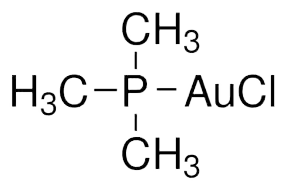
\includegraphics[width=2.2cm]{imagenes/sciFinder/Chloro(trimethylphosphine)gold(I).png} \\
%         \hline
%         & & [Cl-][Au+][P](C=1C=CC=CC1C=2C=CC=CC2) (C(C)(C)C)C(C)(C)C & & 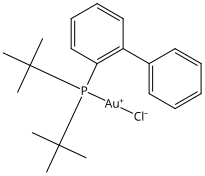
\includegraphics[width=2.2cm]{imagenes/sciFinder/Chloro[(1,1-biphenyl-2-yl)di-tert-butylphosphine]gold(I).png} \\
%         \hline
%         & & O\#C[Fe+2]1234([I-])(C\#O)[CH]=5[CH]4 =[CH]3[CH-]2[CH]51 & & 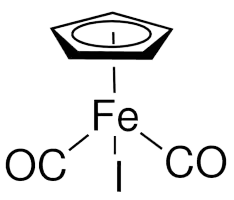
\includegraphics[width=2.2cm]{imagenes/sciFinder/Dicarbonylcyclopentadienyliodoiron(II).png} \\
%         \hline




%         & & O\#C[Fe+2]1234([I-])(C\#O)[CH]=5[CH]4 =[CH]3[CH-]2[CH]51 & & 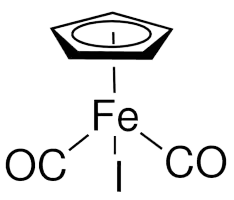
\includegraphics[width=2.2cm]{imagenes/sciFinder/Dicarbonylcyclopentadienyliodoiron(II).png} \\
%         \hline
%         & & O\#C[Fe+2]1234([I-])(C\#O)[CH]=5[CH]4 =[CH]3[CH-]2[CH]51 & & 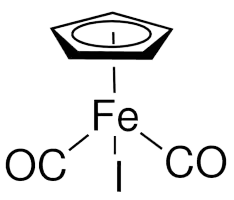
\includegraphics[width=2.2cm]{imagenes/sciFinder/Dicarbonylcyclopentadienyliodoiron(II).png} \\
%         \hline
%         & & O\#C[Fe+2]1234([I-])(C\#O)[CH]=5[CH]4 =[CH]3[CH-]2[CH]51 & & 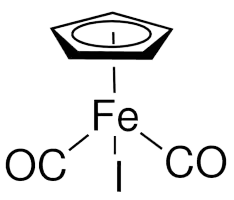
\includegraphics[width=2.2cm]{imagenes/sciFinder/Dicarbonylcyclopentadienyliodoiron(II).png} \\
%         \hline
%         & & O\#C[Fe+2]1234([I-])(C\#O)[CH]=5[CH]4 =[CH]3[CH-]2[CH]51 & & 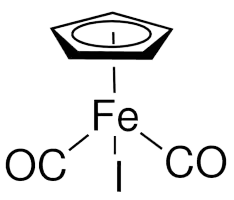
\includegraphics[width=2.2cm]{imagenes/sciFinder/Dicarbonylcyclopentadienyliodoiron(II).png} \\
%         \hline
%         & & O\#C[Fe+2]1234([I-])(C\#O)[CH]=5[CH]4 =[CH]3[CH-]2[CH]51 & & 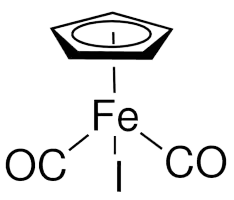
\includegraphics[width=2.2cm]{imagenes/sciFinder/Dicarbonylcyclopentadienyliodoiron(II).png} \\
%         \hline

%         \end{tabular}
%     \caption{Tabla extendida para el set de datos de 30 moléculas. Contiene el nombre del compuesto (uno de los varios sinónimos según el formato de nomenclatura de la IUPAC), la cadena SMILES extraída de Sigma-Aldrich (SA), la cadena SMILES extraída de SciFinder (SF), y las imágenes de las respectivas bases de datos (SA y SF)}
%     \label{tabla:tabla_grande_intro_label}
% \end{table}




\begin{longtable}{m{7cm}m{8cm}cc}
\caption{Tabla extendida para el set de datos de 30 moléculas. Contiene la cadena SMILES extraída de Sigma-Aldrich (SA), la cadena SMILES extraída de SciFinder (SF), y las imágenes de las respectivas bases de datos (SA y SF)}\\
\hline
\textbf{SMILES SA} & \textbf{SMILES SF} & \textbf{Imagen SA} & \textbf{Imagen SF} \\ \hline
\endfirsthead

\multicolumn{4}{c}%
{{\bfseries \tablename\ \thetable{} -- Continuación de la tabla en la página siguiente}} \\
\hline
\textbf{SMILES SA} & \textbf{SMILES SF} & \textbf{Imagen SA} & \textbf{Imagen SF} \\ \hline
\endhead

\hline \multicolumn{4}{r}{{Continúa en la siguiente página}} \\
\endfoot

\hline
\endlastfoot

% Compuesto 2
 C[Au].c1ccc(cc1)P(c2ccccc2) c3ccccc3 & 
 [Au+]([CH3-])[P](C=1C=CC=CC1) (C=2C=CC=CC2)C=3C=CC=CC3 & 
 \includegraphics[width=2.2cm]{imagenes/sigmaAldrich/Methyl(triphenylphosphine)gold(I).png} & 
 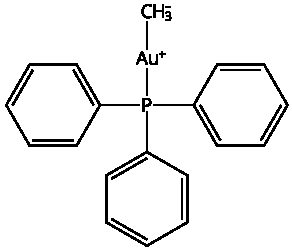
\includegraphics[width=2.2cm]{imagenes/sciFinder/pdf/Methyl(triphenylphosphine)gold(I).pdf} \\
\hline

% Compuesto 3
 Br[Pd]Br.c1ccc(cc1) P(c2ccccc2)c3ccccc3.c4ccc(cc4) P(c5ccccc5)c6ccccc6 & 
 [Br-][Pd+2]([Br-])([P](C=1C= CC=CC1)(C=2C=CC=CC2) C=3C=CC=CC3)[P](C=4C=CC=CC4) (C=5C=CC= CC5)C=6C=CC=CC6 & 
 
\includegraphics[width=2.2cm]{imagenes/placeholder.png} & 
 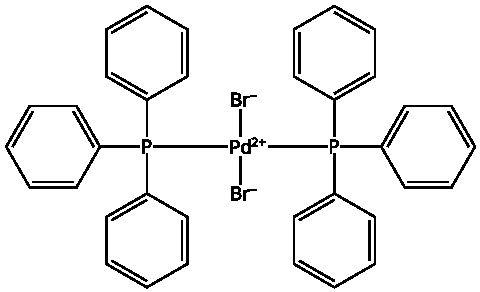
\includegraphics[width=2.2cm]{imagenes/sciFinder/pdf/trans-Dibromobis(triphenylphosphine)palladium(II).pdf} \\
\hline

% Compuesto 4
 Cl[Pd]Cl.C1CC=CCCC=C1 & 
 [Cl-][Pd+2]123([Cl-]) [CH]=4CC[CH]3=[CH]2CC[CH]41 & 
 \includegraphics[width=2.2cm]{imagenes/sigmaAldrich/Dichloro(1,5-cyclooctadiene)palladium(II).png} & 
 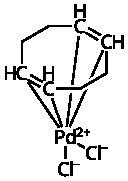
\includegraphics[width=2.2cm]{imagenes/sciFinder/pdf/Dichloro(1,5-cyclooctadiene)palladium(II).pdf} \\
\hline

% Compuesto 5
 C1C[C@@H]2C[C@H]1CC2PC3C [C@@H]4CC[C@H]3C4.CN(C)c5ccccc5-c6ccccc6[Pd]Cl & 
 [Cl-][Pd+2]1([C-]=2C=CC=CC2C=3C =CC=CC3[N]1(C)C)[PH] (C4CC5CCC4C5)C6CC7CCC6C7 & 
 
\includegraphics[width=2.2cm]{imagenes/placeholder.png} & 
 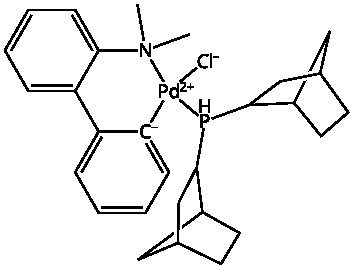
\includegraphics[width=2.2cm]{imagenes/sciFinder/pdf/SK-CC 01A.pdf} \\
\hline

% Compuesto 6
 C\textbackslash C(=N/O)c1ccc(O)cc1[Pd]Cl .C\textbackslash C(=N/O)c2ccc(O)cc2[Pd]Cl & 
 OC=1C=CC=2C(=[N](O)[Pd+2]3 ([Cl-][Pd+2]4([Cl-]3)[C-]=5 C=C(O)C=CC5C(=[N]4O)C)[C-]2C1)C & 
 
\includegraphics[width=2.2cm]{imagenes/placeholder.png} & 
 \includegraphics[width=2.2cm]{imagenes/sciFinder/pdf/Bis[µ-chloro[5-hydroxy-2-[1-(hydroxyimino)ethyl]phenyl]palladium].pdf} \\
\hline


% Compuesto 7
 No se encontró el compuesto en Sigma-Aldrich & 
 FC=1C(Cl)=C(F)[C-](=C(F)C1Cl)[Pd+2] ([I-])([As](C=2C=CC=CC2)(C=3C=CC=C C3)C=4C=CC=CC4)[As](C=5C=CC=CC5) (C=6C=CC=CC6)C=7C=CC=CC7 & 
 
\includegraphics[width=2.2cm]{imagenes/placeholder.png} & 
 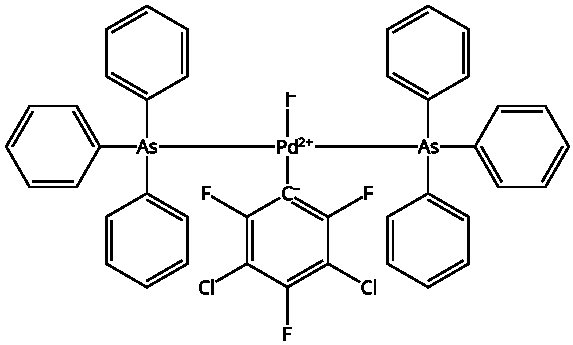
\includegraphics[width=2.5cm]{imagenes/sciFinder/pdf/(SP-4-3)-(3,5-Dichloro-2,4,6-trifluorophenyl)iodobis(triphenylarsine)palladium.pdf} \\
\hline


% Compuesto 8
 No se encontró el compuesto en Sigma-Aldrich & 
 O=S(=O)([NH-][Pd+4]12([F-])([C-]=3C=CC=CC3C(C)(C)[CH2-]1) [N]=4C=CC=CC4C=5C=CC=C[N] 52)C6=CC=C(C=C6)C & 
 
\includegraphics[width=2.2cm]{imagenes/placeholder.png} & 
 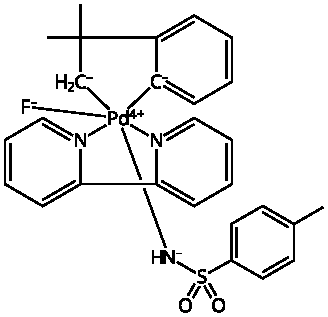
\includegraphics[width=2.2cm]{imagenes/sciFinder/pdf/Palladium, (2,2-bipyridine-κN1,κN1)[(2,2-dimethyl-1,2-ethanediyl)-1,2-phenylene]fluoro(4-methylbenzenesulfonamidato-κN)-, (OC-6-35).pdf} \\
\hline


% Compuesto 9
 Br[Ni]Br.COCCOC & 
 [Br-][Ni+2]1([Br-])O(C)CCO1C & 
 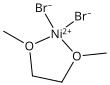
\includegraphics[width=2.2cm]{imagenes/sigmaAldrich/Nickel(II) bromide ethylene glycol dimethyl ether complex.png} & 
 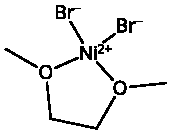
\includegraphics[width=2.2cm]{imagenes/sciFinder/pdf/Dibromo(1,2-dimethoxyethane)nickel(II).pdf} \\
\hline


% Compuesto 10
 Cl[Ru](Cl)(C\#[O])(C\#[O])([PH](c1ccccc1) (c2ccccc2)c3ccccc3)[PH](c4ccccc4) (c5ccccc5)c6ccccc6 & 
 O\#C[Ru+2]([Cl-])([Cl-])(C\#O)([P](C=1C=CC=CC1) (C=2C=CC=CC2)C=3C=CC=CC3)[P] (C=4C=CC=CC4)(C=5C=CC=CC5) C=6C=CC=CC6 & 
 
\includegraphics[width=2.2cm]{imagenes/placeholder.png} & 
 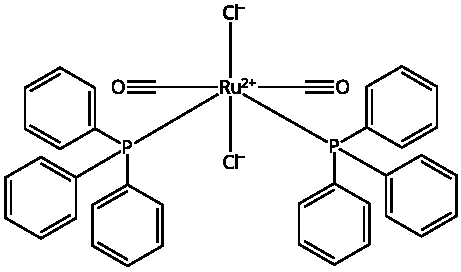
\includegraphics[width=2.2cm]{imagenes/sciFinder/pdf/Bis(triphenylphosphine)ruthenium(II) dicarbonyl chloride.pdf} \\
\hline

% Compuesto 11
 \ldots & 
 \ldots & 
 
\includegraphics[width=2.2cm]{imagenes/placeholder.png} & 
 
\includegraphics[width=2.2cm]{imagenes/placeholder.png} \\
\hline


% Compuesto 12
 \ldots & 
 \ldots & 
 
\includegraphics[width=2.2cm]{imagenes/placeholder.png} & 
 
\includegraphics[width=2.2cm]{imagenes/placeholder.png} \\
\hline



% Compuesto 13
 \ldots & 
 \ldots & 
 
\includegraphics[width=2.2cm]{imagenes/placeholder.png} & 
 
\includegraphics[width=2.2cm]{imagenes/placeholder.png} \\
\hline



% Compuesto 14
 \ldots & 
 \ldots & 
 
\includegraphics[width=2.2cm]{imagenes/placeholder.png} & 
 
\includegraphics[width=2.2cm]{imagenes/placeholder.png} \\
\hline


\end{longtable}

\textbf{POR TEMRINAR}

\end{landscape}


% \includepdf[pages=-, offset=0 0,landscape=true,picturecommand*={\put (\LenToUnit{.05\paperwidth},20) {[1]};}]{Iteracion3/pdfs/planificacion/Planificacion_inicial_iteracion3_21Noviembre2021.pdf}